\documentclass{standalone}

\usepackage{amsmath}
\usepackage{bm}
\usepackage{tikz}
\usetikzlibrary{%
	calc,%
	patterns,%
	decorations.pathreplacing,%
	decorations.pathmorphing,%
	arrows.meta,%
}
\usepackage{pgfplots}
\pgfplotsset{compat=1.16}
\usepackage{stanli}

\usepackage[active, tightpage]{preview}
\PreviewEnvironment{tikzpicture}
\setlength\PreviewBorder{2mm}

\definecolor{BAMred1}{cmyk}{0.10, 1.00, 1.00, 0.00}
\definecolor{BAMred2}{cmyk}{0.30, 1.00, 1.00, 0.00}
\definecolor{BAMred3}{cmyk}{0.25, 1.00, 1.00, 0.35}
\definecolor{BAMblue1}{cmyk}{1.00, 0.00, 0.00, 0.00}
\definecolor{BAMblue2}{cmyk}{1.00, 0.40, 0.35, 0.25}
\definecolor{BAMblue3}{cmyk}{0.75, 0.00, 0.00, 0.80}
\definecolor{BAMblue4}{cmyk}{1.00, 0.70, 0.40, 0.70}
\definecolor{BAMyellow1}{cmyk}{0.00, 0.10, 1.00, 0.00}
\definecolor{BAMyellow2}{cmyk}{0.00, 0.25, 1.00, 0.15}
\definecolor{BAMyellow3}{cmyk}{0.00, 0.20, 1.00, 0.10}
\definecolor{BAMyellow4}{cmyk}{0.05, 0.40, 1.00, 0.20}
\definecolor{BAMgreen1}{cmyk}{0.20, 0.00, 1.00, 0.20}
\definecolor{BAMgreen2}{cmyk}{0.15, 0.00, 1.00, 0.50}
\definecolor{BAMgreen3}{cmyk}{0.75, 0.50, 1.00, 0.00}
\definecolor{BAMgreen4}{cmyk}{0.80, 0.60, 1.00, 0.50}
\definecolor{BAMgrad100}{cmyk}{0.45, 0.00, 0.00, 0.95}
\definecolor{BAMgrad080}{cmyk}{0.36, 0.00, 0.00, 0.76}
\definecolor{BAMgrad050}{cmyk}{0.225,0.00, 0.00, 0.475}
\definecolor{BAMgrad020}{cmyk}{0.09, 0.00, 0.00, 0.19}
\definecolor{BAMgrad010}{cmyk}{0.045, 0.00, 0.00, 0.095}


\newcommand{\DrawTriangle}[3]{% x, y, a
	\draw[] (#1, #2)-- (#1-#3, #2-#3)-- (#1+#3, #2-#3)--cycle;
}
\pgfdeclarelayer{mybg}
\pgfsetlayers{mybg, main}

\begin{document}
\begin{tikzpicture}[
	baseline,
	scale=1.0,
	fixed/.style={
		postaction={draw,decorate,decoration={border,angle=-45,
			    amplitude=0.12cm,segment length=0.5mm}}},
	]
	\tikzstyle{every node}=[font=\Large]
	\def\L{4.0cm}
	\pgfmathsetmacro\M{4.0-0.2}
	\pgfmathsetmacro\EPS{0.00001cm}
	\pgfmathsetmacro\h{\L / 10cm}

	% first put RVE on main layer
	\draw[BAMred2, thick] (0, 0) coordinate (za) -- (\h, 0) coordinate (zb) -- (\h, \h) coordinate (zc) --(0, \h) coordinate (zd) -- cycle;
	\node[inner sep=0] (rce) at (10cm, 1cm) {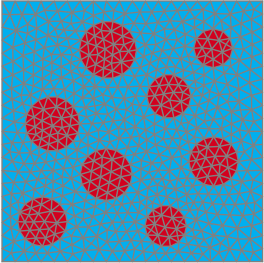
\includegraphics[scale=0.8]{./rce_noaxis_cropped.png}};
	% put everything else on background layer
	\begin{pgfonlayer}{mybg}
		\draw[black, ultra thick, fill=BAMgrad020] (0, 0) -- (\L, 0) -- (\L, \L) -- (-\L, \L) -- (-\L, -\L) -- (0, -\L) -- cycle;
		\DrawTriangle{-\L}{-\L}{0.16cm}
		\draw[black, line width=.5pt, fixed] (-\L-0.15cm, -\L-0.16cm) --+(0.30cm, 0);
		\foreach \x in {0.0, 0.4, 0.8, ..., \M}{
			\DrawTriangle{-\x cm}{-\L}{0.12cm}
			\draw[black, line width=.5pt, fixed] (-\x cm - 0.15cm, -\L-0.16cm) --+(0.3cm, 0.0);
		}
		\draw[ultra thick, stealth-] (\L-\h cm, 0) -- +(0, - 2.5 * \h) coordinate (F) node [right] {$F, \hat{u}$};
		\point{a}{\L}{0.0};
		\point{b}{\L}{\L};
		\dimensioning{2}{a}{b}{-\L-0.4cm}[$200\,\mathrm{mm}$];
		\point{c}{\L}{-\L};
		\dimensioning{2}{c}{a}{-\L-0.4cm}[$200\,\mathrm{mm}$];
		\point{d}{-\L}{-\L-0.5cm};
		\point{e}{0.0}{-\L-0.5cm};
		\dimensioning{1}{d}{e}{-\L-0.75cm}[$200\,\mathrm{mm}$];
		\point{f}{\L-\h cm}{-\L-0.5cm};
		\dimensioning{1}{e}{f}{-\L-0.75cm}[$180\,\mathrm{mm}$];
		\point{g}{\L}{-\L-0.5cm};
		\dimensioning{1}{f}{g}{-\L-0.75cm}[$20\,\mathrm{mm}$];
		% bounding box for alignment
		% \draw (current bounding box.south east) rectangle (current bounding box.north west);
		% somehow pgfonlayer ignores onslide command
		\draw[BAMred2, thick] (za)--(rce.south west);
		\draw[BAMred2, thick] (zb)--(rce.south east);
		\draw[BAMred2, thick] (zc)--(rce.north east);
		\draw[BAMred2, thick] (zd)--(rce.north west);
	\end{pgfonlayer}
\end{tikzpicture}
\end{document}
